
\begin{center}
\Huge
	Harmoniske svingninger
\end{center}
\section*{Harmoniske svingninger}
\stepcounter{section}

Vi har tidligere set graferne for cosinus, sinus og tangens. Disse kan ofte være meningsfulde at skalere og parallelforskyde for at beskrive forskellige periodiske fænomener. Den \textit{harmoniske svingning} defineres ud fra sinus på følgende vis. 
\begin{defn}[Harmonisk svingning]
	Den harmoniske svingning $f$ defineres som funktionen
	\begin{align*}
		f(x) = A\sin(\omega x + \varphi) + B,
	\end{align*}
	hvor
	\begin{enumerate}[label=$\cdot$]
		\item $A$ kaldes amplituden,
		\item $\omega$ kaldes vinkelhastigheden, 
		\item $\varphi$ kaldes faseforskydningen.
		\item $B$ tilsvarer en lodret parallelforskydning.
	\end{enumerate}
\end{defn}
Vi kan se en illustration af en harmonisk svingning på Figur \ref{fig:harmonisk}.
\begin{figure}[H]
	\centering
	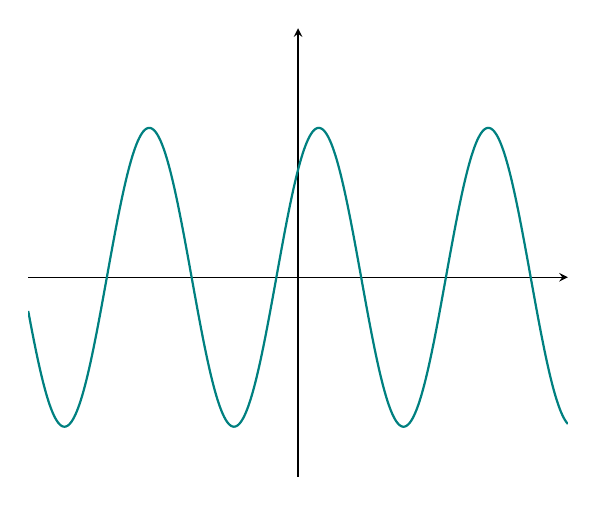
\begin{tikzpicture}
	\begin{axis}
		[
		axis lines = center, 
		xmin = -10, xmax = 10,
		ymin = -2, ymax = 2.5, 
		ticks = none
		]
		\addplot[color = teal, thick, samples = 400, domain = -10:10] {1.5*sin(deg(x+3.1415/4) + 1};
	\end{axis}
	\end{tikzpicture}
	\caption{Graf for harmonisk svingning}
	\label{fig:harmonisk}
\end{figure}
For at se, hvordan vi kan aflæse $A$, $\omega$, $\varphi$ og $B$, betragter vi et eksempel.
\begin{exa}
	Vi ser på funktionen $f$ givet på Figur \ref{fig:exa1}
	\begin{figure}[H]
		\centering
		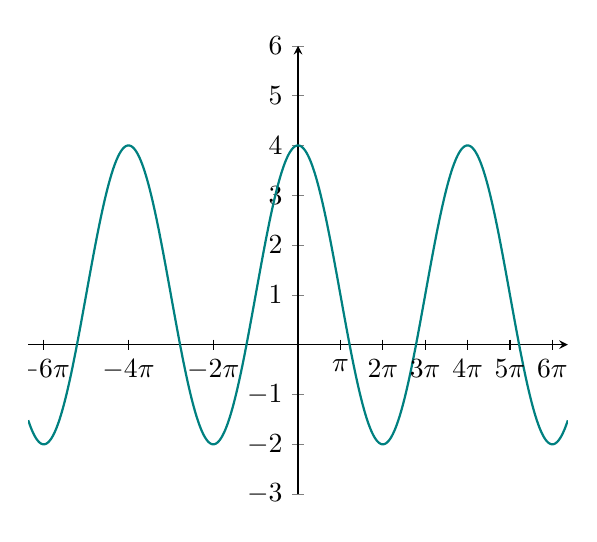
\begin{tikzpicture}
		\begin{axis}
			[
			axis lines = center,
			xmin = -20, xmax = 20,
			ymin = -3, ymax = 6, 
			ytick = {-3,-2,...,5,6},
			xtick = {0},		
			]
			\addplot[color = teal, samples = 1000, domain = -20:20, thick] {3*sin(deg(0.5*x + 3.1415/2)) + 1};
			\draw (axis cs: {3.1415 * (-6)} , 0.1) -- (axis cs: {3.1415 * (-6)} , -0.1)
			node[pos = 1, anchor = north] {$-6\pi$};
		%	\draw (axis cs: {3.1415 * (-5)} , 0.1) -- (axis cs: {3.1415 * (-5)} , -0.1)
		%	node[pos = 1, anchor = north] {$-5\pi$};			
			\draw (axis cs: {3.1415 * (-4)} , 0.1) -- (axis cs: {3.1415 * (-4)} , -0.1)
			node[pos = 1, anchor = north] {$-4\pi$};
		%	\draw (axis cs: {3.1415 * (-3)} , 0.1) -- (axis cs: {3.1415 * (-3)} , -0.1) 
		%	node[pos = 1, anchor = north] {$-3\pi$};
			\draw (axis cs: {3.1415 * (-2)} , 0.1) -- (axis cs: {3.1415 * (-2)} , -0.1)
			node[pos = 1, anchor = north] {$-2\pi$};
		%	\draw (axis cs: {3.1415 * (-1)} , 0.1) -- (axis cs: {3.1415 * (-1)} , -0.1)
		%	node[pos = 1, anchor = north] {$-\pi$};
			\draw (axis cs: {3.1415 * (1)} , 0.1) -- (axis cs: {3.1415 * (1)} , -0.1)
			node[pos = 1, anchor = north] {$\pi$};
			\draw (axis cs: {3.1415 * (2)} , 0.1) -- (axis cs: {3.1415 * (2)} , -0.1)
			node[pos = 1, anchor = north] {$2\pi$};
			\draw (axis cs: {3.1415 * (3)} , 0.1) -- (axis cs: {3.1415 * (3)} , -0.1)
			node[pos = 1, anchor = north] {$3\pi$};
			\draw (axis cs: {3.1415 * (4)} , 0.1) -- (axis cs: {3.1415 * (4)} , -0.1)
			node[pos = 1, anchor = north] {$4\pi$};
			\draw (axis cs: {3.1415 * (5)} , 0.1) -- (axis cs: {3.1415 * (5)} , -0.1)
			node[pos = 1, anchor = north] {$5\pi$};
			\draw (axis cs: {3.1415 * (6)} , 0.1) -- (axis cs: {3.1415 * (6)} , -0.1)
			node[pos = 1, anchor = north] {$6\pi$};
		\end{axis}
		\end{tikzpicture}
		\caption{Graf for $f$.}
		\label{fig:exa1}
	\end{figure}
	Vi ved, at $\sin$ går fra $-1$ til $1$, så da grafen for $f$ går fra $-2$ til $4$, så har værdimængden 
	en intervalbredde på 6 i stedet for 2, så $A = 3$. Intervalmidtpunktet er 1, så $B = 1$. 
	$\sin(0)$ og $\sin\left(\frac{\pi}{2}\right) = 1$, så vi kan se, at grafen er parallelforskudt $\frac{\pi}{2}$ til
	 venstre og $\varphi = \frac{\pi}{2}$.
	Afslutningsvist kan vi se, at $\sin$ normalt har en periode på $2\pi$, altså at
	$\sin(x + 2\pi) = \sin(x)$, men perioden for $f$ er $4\pi$, så $\omega = 0.5$. 
\end{exa}
For harmoniske svingninger kan vi finde perioden som 
\begin{align*}
	T = \frac{2\pi}{\omega}
\end{align*}
Dette stemmer også overens med eksemplet, hvor perioden er 
\begin{align*}
	T = \frac{2\pi}{0.5} = 4\pi
\end{align*}
\subsection*{Opgave 1}
Tegn grafen for $f$ givet ved
\begin{align*}
	f(x) = A\sin(\omega x + \varphi) + B
\end{align*}
I GeoGebra, hvor du laver skydere til $A$, $\omega$, $\varphi$ og $B$. Find ud af, hvad konstanterne hver i sær gør ved grafen. 

\subsection*{Opgave 2}
Bestem perioden for følgende harmoniske svingninger.
\begin{enumerate}[label=\roman*)]
	\item $f(x) = 10\sin(x + 2\pi)$
	\item $f(x) = 2\sin(4x)$
	\item $f(x) = 5\sin(0.1x + 13)-1$
	\item $f(x) = \sin(8x +1)-12$
\end{enumerate}
\subsection*{Opgave 3}
Bestem konstanterne $A$, $B$, $\omega$ og $\varphi$ for følgende harmoniske svingninger.
Bestem desuden perioden $T$.
\begin{center}
		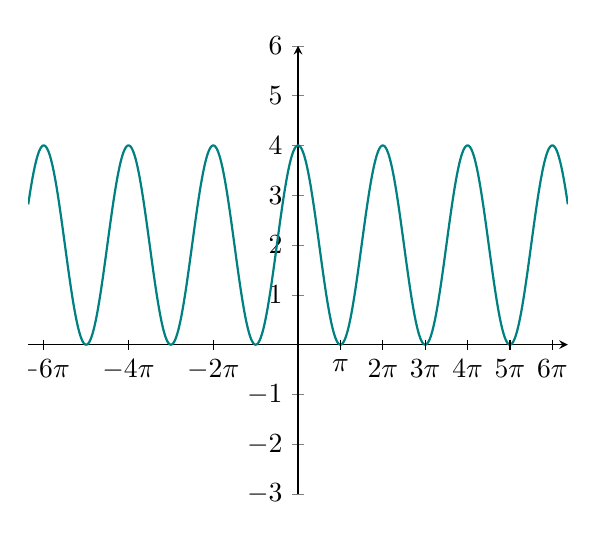
\begin{tikzpicture}
		\begin{axis}
			[
			axis lines = center,
			xmin = -20, xmax = 20,
			ymin = -3, ymax = 6, 
			ytick = {-3,-2,...,5,6},
			xtick = {0},		
			]
			\addplot[color = teal, samples = 1000, domain = -20:20, thick] {2*sin(deg(x + 3.1415/2)) + 2};
			\draw (axis cs: {3.1415 * (-6)} , 0.1) -- (axis cs: {3.1415 * (-6)} , -0.1)
			node[pos = 1, anchor = north] {$-6\pi$};
		%	\draw (axis cs: {3.1415 * (-5)} , 0.1) -- (axis cs: {3.1415 * (-5)} , -0.1)
		%	node[pos = 1, anchor = north] {$-5\pi$};			
			\draw (axis cs: {3.1415 * (-4)} , 0.1) -- (axis cs: {3.1415 * (-4)} , -0.1)
			node[pos = 1, anchor = north] {$-4\pi$};
		%	\draw (axis cs: {3.1415 * (-3)} , 0.1) -- (axis cs: {3.1415 * (-3)} , -0.1) 
		%	node[pos = 1, anchor = north] {$-3\pi$};
			\draw (axis cs: {3.1415 * (-2)} , 0.1) -- (axis cs: {3.1415 * (-2)} , -0.1)
			node[pos = 1, anchor = north] {$-2\pi$};
		%	\draw (axis cs: {3.1415 * (-1)} , 0.1) -- (axis cs: {3.1415 * (-1)} , -0.1)
		%	node[pos = 1, anchor = north] {$-\pi$};
			\draw (axis cs: {3.1415 * (1)} , 0.1) -- (axis cs: {3.1415 * (1)} , -0.1)
			node[pos = 1, anchor = north] {$\pi$};
			\draw (axis cs: {3.1415 * (2)} , 0.1) -- (axis cs: {3.1415 * (2)} , -0.1)
			node[pos = 1, anchor = north] {$2\pi$};
			\draw (axis cs: {3.1415 * (3)} , 0.1) -- (axis cs: {3.1415 * (3)} , -0.1)
			node[pos = 1, anchor = north] {$3\pi$};
			\draw (axis cs: {3.1415 * (4)} , 0.1) -- (axis cs: {3.1415 * (4)} , -0.1)
			node[pos = 1, anchor = north] {$4\pi$};
			\draw (axis cs: {3.1415 * (5)} , 0.1) -- (axis cs: {3.1415 * (5)} , -0.1)
			node[pos = 1, anchor = north] {$5\pi$};
			\draw (axis cs: {3.1415 * (6)} , 0.1) -- (axis cs: {3.1415 * (6)} , -0.1)
			node[pos = 1, anchor = north] {$6\pi$};
		\end{axis}
		\end{tikzpicture}
		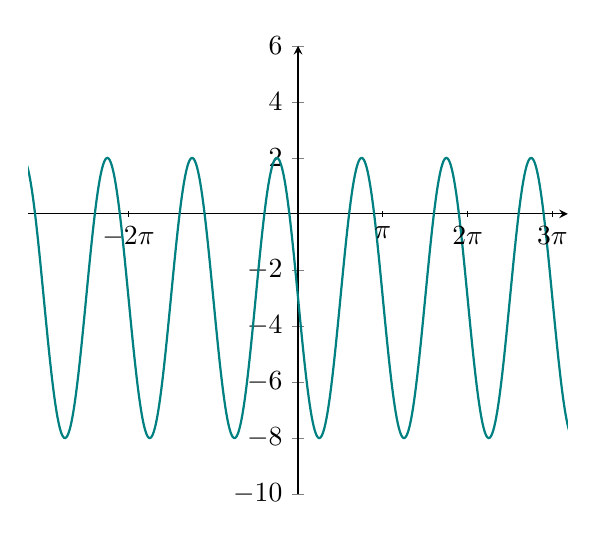
\begin{tikzpicture}
		\begin{axis}
			[
			axis lines = center,
			xmin = -10, xmax = 10,
			ymin = -10, ymax = 6, 
			ytick = {-12,-10,...,10,12},
			xtick = {0},		
			]
			\addplot[color = teal, samples = 1000, domain = -20:20, thick] {5*sin(deg(2*x+ 3.1415)) -3};
			\draw (axis cs: {3.1415 * (-6)} , 0.1) -- (axis cs: {3.1415 * (-6)} , -0.1)
			node[pos = 1, anchor = north] {$-6\pi$};
		%	\draw (axis cs: {3.1415 * (-5)} , 0.1) -- (axis cs: {3.1415 * (-5)} , -0.1)
		%	node[pos = 1, anchor = north] {$-5\pi$};			
			\draw (axis cs: {3.1415 * (-4)} , 0.1) -- (axis cs: {3.1415 * (-4)} , -0.1)
			node[pos = 1, anchor = north] {$-4\pi$};
		%	\draw (axis cs: {3.1415 * (-3)} , 0.1) -- (axis cs: {3.1415 * (-3)} , -0.1) 
		%	node[pos = 1, anchor = north] {$-3\pi$};
			\draw (axis cs: {3.1415 * (-2)} , 0.1) -- (axis cs: {3.1415 * (-2)} , -0.1)
			node[pos = 1, anchor = north] {$-2\pi$};
		%	\draw (axis cs: {3.1415 * (-1)} , 0.1) -- (axis cs: {3.1415 * (-1)} , -0.1)
		%	node[pos = 1, anchor = north] {$-\pi$};
			\draw (axis cs: {3.1415 * (1)} , 0.1) -- (axis cs: {3.1415 * (1)} , -0.1)
			node[pos = 1, anchor = north] {$\pi$};
			\draw (axis cs: {3.1415 * (2)} , 0.1) -- (axis cs: {3.1415 * (2)} , -0.1)
			node[pos = 1, anchor = north] {$2\pi$};
			\draw (axis cs: {3.1415 * (3)} , 0.1) -- (axis cs: {3.1415 * (3)} , -0.1)
			node[pos = 1, anchor = north] {$3\pi$};
			\draw (axis cs: {3.1415 * (4)} , 0.1) -- (axis cs: {3.1415 * (4)} , -0.1)
			node[pos = 1, anchor = north] {$4\pi$};
			\draw (axis cs: {3.1415 * (5)} , 0.1) -- (axis cs: {3.1415 * (5)} , -0.1)
			node[pos = 1, anchor = north] {$5\pi$};
			\draw (axis cs: {3.1415 * (6)} , 0.1) -- (axis cs: {3.1415 * (6)} , -0.1)
			node[pos = 1, anchor = north] {$6\pi$};
		\end{axis}
		\end{tikzpicture}
		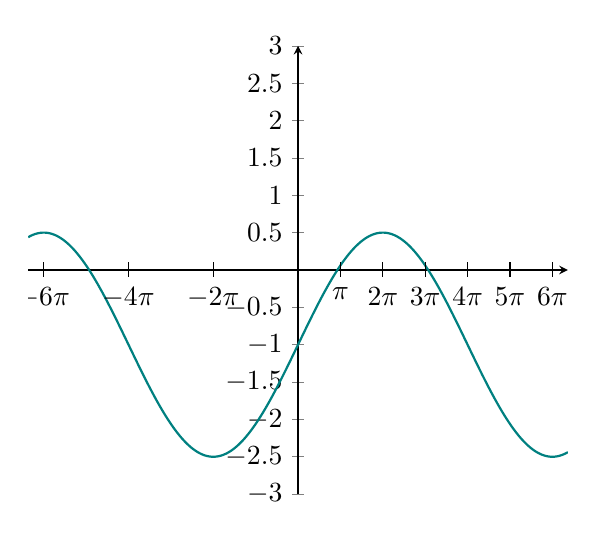
\begin{tikzpicture}
		\begin{axis}
			[
			axis lines = center,
			xmin = -20, xmax = 20,
			ymin = -3, ymax = 3, 
			ytick = {-12,-11.5,...,11.5,12},
			xtick = {0},		
			]
			\addplot[color = teal, samples = 1000, domain = -20:20, thick] {1.5*sin(deg(0.25*x))  -1};
			\draw (axis cs: {3.1415 * (-6)} , 0.1) -- (axis cs: {3.1415 * (-6)} , -0.1)
			node[pos = 1, anchor = north] {$-6\pi$};
		%	\draw (axis cs: {3.1415 * (-5)} , 0.1) -- (axis cs: {3.1415 * (-5)} , -0.1)
		%	node[pos = 1, anchor = north] {$-5\pi$};			
			\draw (axis cs: {3.1415 * (-4)} , 0.1) -- (axis cs: {3.1415 * (-4)} , -0.1)
			node[pos = 1, anchor = north] {$-4\pi$};
		%	\draw (axis cs: {3.1415 * (-3)} , 0.1) -- (axis cs: {3.1415 * (-3)} , -0.1) 
		%	node[pos = 1, anchor = north] {$-3\pi$};
			\draw (axis cs: {3.1415 * (-2)} , 0.1) -- (axis cs: {3.1415 * (-2)} , -0.1)
			node[pos = 1, anchor = north] {$-2\pi$};
		%	\draw (axis cs: {3.1415 * (-1)} , 0.1) -- (axis cs: {3.1415 * (-1)} , -0.1)
		%	node[pos = 1, anchor = north] {$-\pi$};
			\draw (axis cs: {3.1415 * (1)} , 0.1) -- (axis cs: {3.1415 * (1)} , -0.1)
			node[pos = 1, anchor = north] {$\pi$};
			\draw (axis cs: {3.1415 * (2)} , 0.1) -- (axis cs: {3.1415 * (2)} , -0.1)
			node[pos = 1, anchor = north] {$2\pi$};
			\draw (axis cs: {3.1415 * (3)} , 0.1) -- (axis cs: {3.1415 * (3)} , -0.1)
			node[pos = 1, anchor = north] {$3\pi$};
			\draw (axis cs: {3.1415 * (4)} , 0.1) -- (axis cs: {3.1415 * (4)} , -0.1)
			node[pos = 1, anchor = north] {$4\pi$};
			\draw (axis cs: {3.1415 * (5)} , 0.1) -- (axis cs: {3.1415 * (5)} , -0.1)
			node[pos = 1, anchor = north] {$5\pi$};
			\draw (axis cs: {3.1415 * (6)} , 0.1) -- (axis cs: {3.1415 * (6)} , -0.1)
			node[pos = 1, anchor = north] {$6\pi$};
		\end{axis}
		\end{tikzpicture}
	\end{center}	
\subsection*{Opgave 4}
Skitsér grafen for $f$ på $-2\pi \leq x \leq 3\pi$ givet ved
\begin{align*}
	f(x) = A\sin(\omega x + \varphi) + B
\end{align*}	
For følgende valg af $A$, $\omega$, $\varphi$ og $B$. 
\begin{enumerate}[label=\roman*)]
	\item $A = 1$, $\omega = 1$, $\varphi = \pi$, $B = 0$.
	\item $A = 2$, $\omega = \frac{1}{2}$, $\varphi = \frac{\pi}{2}$, $B = 2$.\\
	\item $A = 4$, $\omega = 2$, $\varphi = \frac{-\pi}{2}$, $B = -3$.\\
	\item $A = 6$, $\omega = \frac{1}{4}$, $\varphi = -\pi$, $B = 1$.
\end{enumerate}

\subsection*{Opgave 5}
Hvilket tal skal vi vælge for $\varphi$ for at $\sin(x + \varphi) = \cos(x)$. 

\subsection*{Opgave 6 (Med hjælpemidler)}
Grafen for $f$ givet ved
\begin{align*}
	f(x) = A\sin(\omega x + \varphi) + B
\end{align*}
har to på hinanden følgende ekstrema. Det første er et maksimum i (4,10) og det næste er et minimum i (10,-5).
\begin{enumerate}[label=\roman*)]
	\item Bestem tallene $A$, $\omega$, $\varphi$ og $B$. 
\end{enumerate}

\subsection*{Opgave 7}
En harmonisk svingning har
\begin{enumerate}[label=$\circ$]
	\item Maksimum i 2 og minimum i $-12$,
	\item Går gennem $(0,0)$,
	\item Har periode på $8\pi$.
\end{enumerate} 
Bestem en forskrift for $f$. 
